\documentclass[12pt]{standalone}
\usepackage{tikz}
\usetikzlibrary{calc, patterns} % arrows.meta, decorations.pathreplacing}

\begin{document}


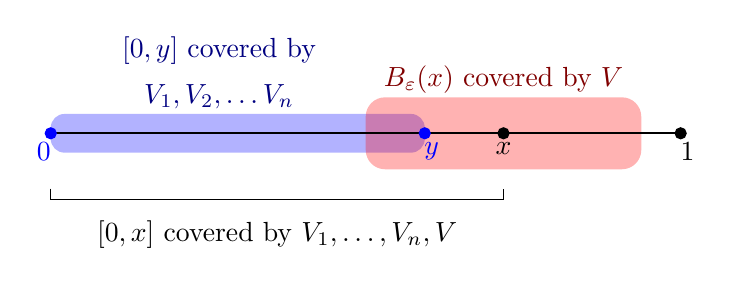
\begin{tikzpicture}
	\coordinate (O) at (-2,0);
	\coordinate (x) at (3.75, 0);
	\coordinate (z) at (2.75, 0);
	\coordinate (P) at (6, 0);
	\def\r{1.75}
	\colorlet{zcolor}{blue}
	\colorlet{acolor}{red}
\fill[fill=zcolor, fill opacity=0.3, rounded corners=5pt] ($(O) + (0, -7pt)$) rectangle ($(z) + (0, 7pt)$)
	 node[zcolor!50!black, text opacity=1.0, pos=0.45, above=22pt]{$[0,y]$ covered by}
	 node[zcolor!50!black, text opacity=1.0, pos=0.45, above=6pt]{$V_1, V_2,\dots V_n$};
\fill[fill=acolor, fill opacity=0.3, rounded corners=7pt] ($(x) + (-\r, -13pt)$) rectangle ($(x) + (\r, 13pt)$)
	 % node[acolor!50!black, text opacity=1.0, pos=0.5, above=27pt]{$(x-\varepsilon,x+\varepsilon)$}
	 node[acolor!50!black, text opacity=1.0, pos=0.5, above=11pt]{$B_\varepsilon(x)$ covered by $V$};
	\draw[thick] (O) -- (P);
			% \draw[blue, very thick] (-2,0) -- (2,0);
			% \draw[{Parenthesis[]}-, blue, very thick, shorten >= 1pt] (2,0)  -- (3.5, 0);
			% \draw[-{Parenthesis[]}, red, very thick, shorten <= 1pt] (3.5,0) -- (5, 0);
			% \draw[red, very thick] (5,0) -- (6,0);
			% \draw[thick] (3.5,0) circle(2pt) node[below]{$a$};
			\filldraw[black] (x) circle(2pt) node[below]{$x$};
			\filldraw[blue] (O) circle(2pt)
			node[below,xshift=-2.5pt]{$0$};
			\filldraw[blue] (z) circle(2pt)
			node[below,xshift=2.5pt]{$y$};
			% \filldraw[red, fill=red, thick] (4.25,0) circle(2pt) node[below]{$y$};
			\filldraw[black] (P) circle(2pt)
			node[below, xshift=2.5pt]{$1$};
% \draw[thick, decoration={brace,raise=15pt},decorate, black] (2,0) -- node[above=34pt]{$(a-\varepsilon, a+\varepsilon)$} node[above=20pt, anchor=south]{ covered by $W$}(5,0);


% \draw[thick, decoration={brace,raise=20pt},decorate, blue] (2.75,0) -- node[below=25pt, anchor=north]{covered by $W_1,W_2,\dots,W_n$}(-2, 0);

\draw[black] ($(O) + (0,-20pt)$) -- ($(O) + (0,-24pt)$) -- 
	 node[black, text opacity=1.0, pos=0.5, below=4pt]{$[0,x]$ covered by $V_1,\dots,V_n,V$}
($(x) + (0,-24pt)$) -- ($(x) + (0,-20pt)$);
		\end{tikzpicture}
\end{document}
